So as dicussed in the last section \ref{sec:business-process}, the system required a huge
amount of functionalities with a lot of dependencies between them.

So the team came up with the services shown in the following figure
\ref{fig:backend_services} which are hosted  on AWS implementing an SOA architecture.
The SaaS relies on various managed services provided by AWS, such as EC2, S3, RDS, etc.

\begin{figure}[!htpb]
    \centering
    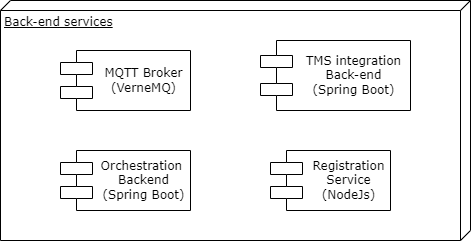
\includegraphics[width=0.65\textwidth]{images/Backend}
    \caption{\footnotesize{Backend services}}
    \label{fig:backend_services}
\end{figure}

The MMSoft Saas is constituted of:
\begin{itemize}
    \item Four front-end services:
    \begin{itemize}
        \item Easy-truck-in (ETI) interface which is the main interface
        \item Driver application (Angular 11)
        \item Registration Tablet App (React 16)
        \item Gatekeeper App (Cermate)
    \end{itemize}
    \item Four Back-end services:
    \begin{itemize}
        \item MQTT Broker communicating with the Gatekeeper app (VerneMQ)
        \item Orchestration Back-end Service (Java 11 Spring Boot 2.6) used by the ETI interface
        \item Registration Service (Node JS 16) used by the Registration Tablet App
        \item TMS Registration Back-end which exposes REST API for integration (Java 11 Spring Boot 2.6)
    \end{itemize}
    \item Two databases:
    \begin{itemize}
        \item MySQL for users, site, configuration
        \item Redis as a database for Daily/Weekly data and for messaging communication with other services
    \end{itemize}
\end{itemize}

\begin{figure}[!htpb]
    \centering
    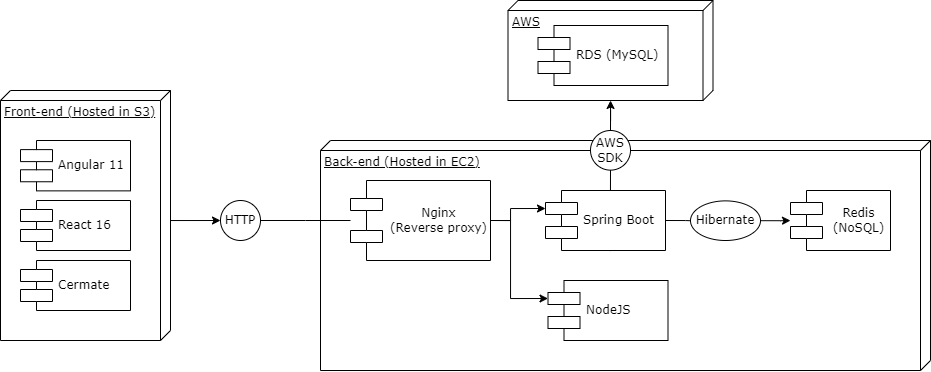
\includegraphics[width=\textwidth]{images/State-of-art}
    \caption{\footnotesize{Current state of the application}}
    \label{fig:state-of-art}
\end{figure}

These following services came in the developed as illustrated
in the following figure \ref{fig:state-of-art}

It's a solution that is fully hosted on AWS services.
Firstly the backend in hosted on EC2, which is a managed service provided by AWS for
hosting virtual Linux machines with a lot of security features and routing capabilities
to isolate the backend services from the rest of the network.

Then the backend services are built in two technologies as discussed the last paragraph:
    \begin{itemize}
        \item Java 11 Spring Boot 2.6
        \item Node JS 16
    \end{itemize}

Those services are interacting with two different databases, the first one being
the MySQL database which holds data for users and sites.
And the second one being Redis which is charge of all real-time data, leading to a better
orchestrated interaction within the system.
Also there's the MQTT broker which is used to communicate with different actors within 
the system such as the gatekeepers, management desk and drivers.

Then there are the front-end services which are based on different frameworks depending 
on the needs of the application:
    \begin{itemize}
        \item Angular 11
        \item React 16
        \item Cermate
    \end{itemize}

For the front-end services, they are being hosted within S3 file storage, which is 
a managed service mainly used for storing files.

And all of those services represent our MVP, which is a result of multiple iterations
of the development process.
